\is{Do we need a couple of introductory sentences to justify why we are concentrating on the technique proposed in [2]?}

\emph{Review:}  In the
linearization based flowpipe computation proposed by Althoff
et. al.~\cite{althoff2008reachability}, at any time $t$ where
$\tr{X}{t} = \init$, first a linear system overapproximation
$\rb{\inf\rb{\stmat{f}{\Omega}{U}},
\inf\rb{\inpmat{f}{\Omega}{U}},U,\err{f}{\Omega}{U}}$  of the
nonlinear system $H$ is computed in a neighborhood $\Omega$ of
$\init$.  The set $\Omega$ is computed as a crude over-approximation
of the reachable set between $[0,t+\delta]$ for a small $\delta$, like
the interval over-approximation in Lemma~\ref{lem:bloat}.  Then, a
more accurate flowpipe is computed based
on the linearized dynamics.  Therefore, the accuracy of flowpipe
$\tr{X}{[t,t+\delta]}$ is positively correlated with the Taylor error
in linearization $\taylor{f}{\Omega}{U}$ in the region $\Omega$.
Since $\Omega$ is a small neighborhood of $\init$, this Taylor error
is close to \is{closely?} correlated with the Taylor error
$\taylor{f}{\overline{\init}}{U}$ inside an interval
overapproximation $\overline{\init}$ of $\init$.  The Taylor error
inside $\overline{\init}$ is positively correlated with the bounds of
$\overline{\init}$ based an Equation in~\ref{eqn:linearize}.
Therefore,~\cite{althoff2008reachability} proposed to reduce the
linearization error by dividing the reachable set $\init$ into smaller
sets based on a performance index and computing the next flowpipe as
the union of flowpipes.  However, the union method
in~\cite{althoff2008reachability} has an important drawback, explained
below.  We address this drawback by using intersection of unions
instead of just the union.
%
\subsection{Motivation for intersection of unions}
\is{I think this subsection should start from the beginning of this section.}
In Althoff. et. al~\cite{althoff2008reachability}, a reachable set
$\init$ is divided into two sets $\init_1$ and $\init_2$ which
minimizes the following quantity for a user chosen normalization error
$\rho\in\reals^n_{>0}$.
%
\begin{align*}
\sup_{i=1}^n\frac{{\sup{\taylor{f}{\overline{\init_1}}{U}}}_i}{\rho_i}\sup_{i=1}^n\frac{\sup{\taylor{f}{\overline{\Omega_2}}{U}}_i}{\rho_i}.~~\text{~\cite{althoff2008reachability}}~\numberthis\label{eqn:pi}
\end{align*}
%
For obtaining smaller divisions, the above pairwise division is used
recursively.

\emph{Drawback:}  Since the Taylor error
$\taylor{f}{\overline{\init}}{U}$ is a multi-dimensional vector, minimizing its
bounds $\sup{\taylor{f}{\overline{\init}}{U}}$ is a multi-objective optimization
problem which does not have a single best solution.  But the above
performance index is a one dimensional measure of the overall
linearization error.  Minimizing this one dimensional performance
index does not necessarily reduce signifcantly the linearization error
along all coordinates.  For illustration, let us consider the
nonlinear system in Example~\ref{eg:ill}.  Let $\init =
[-1,1]\times[-0.5,0.5]\times[-0.1,0.1]$ be the reachable set at a time
point and we take the linearization error before splitting $\rho
= \taylor{f}{\init}{U}$ as the normalization error for splitting.
Using the above performance index, we get that $\init$ should be split
along $x$-axis into $\init_1 = [-1,0]\times[-0.5,0.5]\times[-0.1,0.1]$
and $\init_2 = [0,1]\times[-0.5,0.5]\times[-0.1,0.1]$.  However, there
will be very little reduction in the linearization error along
$y$-axis, which least depends on the width along $x$-axis due to the
multiplication coefficient $0.1$ of $xy$ in $f_3$.  Instead, the best
division to minimize the $y$-directional linearization error is to
divide along $y$-coordinate as $\init_1 =
[-1,1]\times[-0.5,0]\times[-0.1,0.1]$ and $\init_2 =
[-1,1]\times[0,0.5]\times[-0.1,0.1]$.  This means reducing the
linearization error using the above performance index need not
significantly reduce the linearization error along all coordinates.
Besides, it is not known how to choose a normalization error $\rho$
for good flowpipe accuracy.

\paragraph{New method:}  In this paper, we propose an better approach
that ensures reduction in the linearization error along each
individual direction in a finite set of directions.  To do so, we
use \emph{intersection of unions} (IoU).  For each direction, we find
an optimized division of the reach set for reducing the linearization
error.  Then we intersect the union sets corresponding to the
optimized division for linearization error along each direction.  This
way, we ensure that the linearization error is significantly reduced
along each direction in the given set of directions.

As a heuristic, we choose the directions as the eigenvectors of the
nonlinear system at the center of the initial set.  Furthermore, we
only divide an interval overapproximation of the reachable set
$\ivflow{H}{\delta}{K}{\epsilon}{X_0}$ in a small time interval
$[0,\delta]$ because of two reasons.
%
\begin{enumerate}
\item Dividing a reach set increases the representation complexity due to
increase in the number of elements in the union.  So, iterative
division of reach set at various time stamps will blow up the
representation complexity.  Therefore, we only divide the reach set
once at the beginning.
\item  A non-interval flowpipe at some time stamp can not
be divided accurately and reduces the accuracy of future flowpipe.
However, since we divide the interval overapproximation of reachable
set at the beginning, i.e., $\ivflow{H}{\delta}{K}{\epsilon}{X_0}$,
this set can be divided accurately.
\end{enumerate}
%
%% Henceforth, we only divide the interval initial set to
%% compute an intersection of unions representation.
%
\subsection{Computing set of optimized division vectors}
Recall that our initial set is the interval denoted $X_0$.  As a part
of an inductive procedure, we first bloat the initial set to compute
an interval overapproximation $\bounds^{\delta}
= \ivflow{H}{\delta}{K}{\epsilon}{X_0}$ of the reachable set in the
interval $[0,\delta]$.  Let us denote the matrix of eigenvectors of
$\inf\rb{\stmat{f}{X_0}{U}}$ as $\eig$.  Our objective is to minimize
the projection of the Taylor error in a small neighborhood of $\bounds^{\delta}$
along each column vector of $\eig$.  For each direction, we have a
optimized way of dividing the interval $\bounds^{\delta}$, denoted by an
integer vector $q$ that represents the number of divisions along each
dimension.  So, for the set of eigenvector, we get a set of optimized
division vectors.  Subsequently, we cast the initial set as
intersection of union of the divisions corresponding to different
optimized division vectors.  Given a vector of positive integer values
$q\in\integers_{>0}^n$, called \emph{division vector}, we define a set
of interval vectors whose union is a close overapproximation of
$\bounds^{\delta}$ with only floating point approximation error, as follows.
%
\begin{align*}
D_q
= & \left\{r_1\times...\times r_n\right.\\
& \left.\st{\forall i\in\set{1,\ldots,n}~\exists k_i\in\set{1,\ldots,q_i}}:~r_i
= \ivmat{\inf\rb{\bounds^\delta_i}}+k_i\frac{\rad{\bounds^\delta}_i}{q_i}\right\}.
\end{align*}
%
For all intervals in $D_q$, an vector upper bound
$\utaylor{f}{U}{\bounds}{q}$ on the magnitude of Taylor error is
$\forall i\in\set{1,\ldots,n}~\rb{\utaylor{f}{U}{\bounds}{q}}_i$
%
\begin{align*}
\sup\rb{\mymatrix{\rad{\bounds^{\delta}}\rb{\diag{q}}^{-1}\\ \rad{U}}^T{\nabla^2
f_i}\rb{\mymatrix{\bounds^{\delta}\\ U}}\mymatrix{\rad{\bounds^{\delta}}\rb{\diag{q}}^{-1}\\ \rad{U}}}.
\end{align*}
%
For any $k\in\set{1,\ldots,n}$, the projection of the  bound
along the $k^{th}$ eigenvector is given by
$\utaylor{f}{U}{\bounds}{q}\eig_{:,k}
= \utaylor{f}{U}{\bounds}{q}\real{\eig_{:,k}}
+ \iota\utaylor{f}{U}{\bounds}{q}\imag{\eig_{:,i}}$.  We select $q$ to
minimize the maximum absolute value of this bound, by using the
following greedy optimization.  Let us consider for any
$i\in\set{1,\ldots,n}$, \mbox{$\omega\rb{q,i}\in\integers^n$}, where $\omega\rb{q,i}_j
= \begin{cases}2q_j & j=i\\ q_j & i\neq j \end{cases}$.

\begin{algorithm}
\caption{Optimizing division vector for $k^{th}$
eigenvector} $q\gets \mymatrix{1,\ldots,1}^T\in\integers^n$\;
\While{$\prod_{j=1}^nq_j<2^\eta$}{
$ind \gets \argmin_{i=1}^n\begin{cases}\rb{\sup\rb{\real{\utaylor{f}{U}{\bounds^\delta}{\omega\rb{q,i}}\eig_{:,k}}}}^2\\
 + \rb{\sup\rb{\imag{\utaylor{f}{U}{\bounds^\delta}{\omega\rb{q,i}}\eig_{:,k}}}}^2\end{cases}$\;
$q\gets \omega\rb{q,ind}$
}
\end{algorithm}
%
Subsequently, we get a set of optimized division vectors corresponding
to different eigenvectors.  We denote this set as as $\dopt{\eta}$ \is{could we use a different symbol? $\dopt{}$ looks like asymptotic complexity.},
where $2^\eta$ is the maximum number of divisions.
%
\begin{example}
Let us consider the nonlinear system $H$ in Example~\ref{eg:ill}.  Let
us consider that $\bounds^\delta = [0,1]^3$ for some small $\delta$
and the maximum number of divisions is $4$, i.e., $\eta = 2$.  The
eigenvectors at the origin are the coordinate vectors $\mymatrix{1 & 0
& 0}^T$, $\mymatrix{0 & 1 & 0}^T$ and $\mymatrix{0 & 0 & 1}^T$.  To
reduce the linearization error along $\mymatrix{1 & 0 & 0}^T$, the
best possible division vector is $\mymatrix{2 & 1 & 2}^T$, i.e.,
divide $x$ and $\theta$ coordinates.  For the direction $\mymatrix{0 &
1 &0}^T$, the optimum division vector is $\mymatrix{1 & 2 & 2}^T$ and
for the direction $\mymatrix{0 & 0 & 1}^T$, the optimum division
vector is $\mymatrix{1 & 1 & 4}^T$.  So, $\dopt{4} = \set{\mymatrix{2
& 1 & 2}^T, \mymatrix{1 & 2 & 2}^T, \mymatrix{1 & 1 & 4}^T}$.  The
three different division vectors results three different kinds of
divisions of $[0,1]^3$ whose intersection is represented as an IoU of
interval zonotopes.
\end{example}
%
\subsection{Casting initial reach set as IoU of
interval zonotopes} For different division vectors, we get different
types of unions which overapproximate the interval $\bounds^\delta$.
So, we can represent $\bounds^\delta$ as intersection of unions (IoU)
of intervals.  \emph{However, other set representations, like
zonotopes~\cite{girard2005reachability}, provide much better
approximation of reachable sets at future time stamps when
linearization is used}.  But if we use zonotopes, we need to recast
$\bounds^\delta$ as intersection of union of zonotopes. However, it is
known that zonotopes do not provide good approximation of intersection
between them~\cite{ghorbal2010logical}, which is required in our IoU
representation.  Therefore, we generalize zonotopes to interval
zonotopes to compute better approximation of intersection between
zonotopes and also soundly approximate floating point computations.
It is defined as follows.
%
\begin{definition}[Interval Zonotope]
Let us consider $l\in\integers_{>0}$, $\gen\in\intervals^{n\times
ln},\cen\in\intervals^{n}$ and $\bounds\in\intervals^n$.  An interval
zonotope of order $l>1$ is the tuple $\rb{\gen,\cen,\bounds}$ which
represents the following set.
%
\begin{align*}
\iz{\gen}{\cen}{\bounds}
= \set{x\in\reals^n \st{\exists \zeta\in[-1,1]^{nl}:~x\in\bounds,~x \in \gen\ivmat{\zeta}+\cen} }
\end{align*}
%
If $\zt = \iz{\gen}{\cen}{\bounds}$, then we represent $\overline{\zt}
= \bounds$.
\end{definition}
%
Before computing the IoU interval zonotope representation of
$\bounds^\delta$, we will discuss a transformation operation on the
interval zonotope that will be used in the IoU recasting and flowpipe
computation.
%
\begin{lemma}[Linear transformation and sum]\label{lem:lintrans}
Let us consider $A\in\intervals^{n\times n}$, $w\in\intervals^n$ and an
interval zonotope $\rb{{\gen},{\cen},{\bounds}}$ of order $l>1$.  Let us
consider $\gen^\prime\in\reals^{n\times nl}$ where 
%
\begin{align*}
& \gen^\prime_{{:,n+1:ln}} = A\gen_{\rb{:,1:(l-1)n}}\\
& \gen^\prime_{{:,1:n}}
= \diag{\sup\rb{\rb{A\gen_{\rb{:,(l-1)n+1:ln}} }[-1,1]^n
+ \rad{w} }}\\
& z = \rb{A\gen}[-1,1]^n + A\cen + w.\\
& \text{Then},~\set{A^\prime x + y\st{x\in\iz{\gen}{\cen}{\bounds}, y\in\bounds,
A^\prime\in A}} \\
& \subseteq \iz{\gen^\prime}{A\cen+\mi{w}}{\meet{\rb{A\bounds + A\cen 
+ w}}{z}}~\numberthis\label{eqn:linMin}
\end{align*}
%
\end{lemma}
%
\begin{proof}
Let us consider $x\in \iz{\gen}{\cen}{\bounds}$ and $y\in w$.  So,
there exists $\zeta\in [-1,1]^n$ such that $x \in \gen\zeta + \cen$ and
also $x\in\bounds$.  Then,
%
\begin{align*}
& Ax + y \in A\gen\zeta + A\cen + y\\
& = A\gen_{{:,1:(l-1)n}}\zeta_{{:,1:(l-1)n}} +
A\gen_{:,{(l-1)n+1:ln}}\zeta_{{(l-1)n+1:ln}} + A\cen + y\\
& \subseteq A\gen_{{:,1:(l-1)n}}\zeta_{{:,1:(l-1)n}} 
 + A\gen_{:,{(l-1)n+1:ln}}[-1,1]^n + A\cen + w\\
& = \gen^\prime_{{:,n+1:ln}}\zeta_{{:,1:(l-1)n}} +
\rb{A\gen_{:,{(l-1)n+1:ln}}[-1,1]^n + \rad{w}} + A\cen +  \mi{w} 
\end{align*}
%
We have $A\gen_{:,{(l-1)n+1:ln}}[-1,1]^n + \rad{w} = \set{\gen^\prime_{:,1:n}\zeta^\prime\st{\zeta^\prime\in[-1,1]^n}}$
So, there exists $\zeta^\prime \in[-1,1]^n$ such that
%
\begin{align*}
& Ax + y =  \gen^\prime_{{:,n+1:ln}}\zeta_{{:,1:(l-1)n}}
+ \gen^\prime_{:,1:n}\zeta^\prime + A\cen + \mi{w}\\
& = \gen\mymatrix{\zeta_{{:,1:(l-1)n}}\\\zeta^\prime} + A\cen + \mi{w}~\numberthis~\label{eqn:pr1}
\end{align*}
%
Also, we get the following two bounds.
%
\begin{align*}
 & Ax + y \in A\gen[-1,1]^n + A\cen + w = z~\numberthis\label{eqn:pr2}\\
 & Ax + y \in A\bounds + A\cen + w~\numberthis\label{eqn:pr3}
\end{align*}
%
By~(\ref{eqn:pr1}),(\ref{eqn:pr2}) and (\ref{eqn:pr3}), we get that
$Ax+y\in\iz{\gen^\prime}{A\cen+\mi{w}}{\meet{\rb{A\bounds + A\cen + w}}{z}}$
\end{proof}
%
For convenience, if $\zt = \iz{\gen}{\cen}{\bounds}$, we denote the
R.H.S of~(\ref{eqn:linMin}) as $\lin{\zt}{A}{w}$.  The $n$-dimensional
interval zonotope of order $l$ which is equivalent to zero is denoted
$\zerozon{n}{l}$.
%
Based on the above lemma, for a division vector $q\in\dopt{\eta}$, we
can closely overapproximate $\bounds^\delta$ as a union of interval zonotopes of
order $l>0$ as $\bigcup_{b\in
D_q}\lin{\zerozon{n}{l}}{\sqb{0}_{n\times n}}{b}$ with only floating
point overapproximation error.  To reduce the Taylor error along each
eigenvector, we store the union corresponding to each optimized
division vector in $\dopt{\eta}$ and take their intersection.  The
resulting intersection of unions is
%
\begin{align*}
\bigcap_{q\in\dopt{\eta}}\bigcup_{b\in
D_q}\lin{\zerozon{n}{l}}{\sqb{0}_{n\times n}}{b}~\numberthis\label{eqn:iouopt}
\end{align*}
%
In a computer, we represent an intersection of unions of interval zonotope sets as above with a matrix of interval zonotope tuples, called \emph{IoU interval zonotope}.
%
\begin{definition}[IoU interval zonotope]
An IoU zonotope $\zt$ is a matrix of interval zonotopes which
represents the set
%
\[
\ztset{\zt} = \bigcap_{i=1}^{\rows{\zt}}\bigcup_{i=1}^{\cols{\zt}}\ztset{\zt_{ij}}.
\]
%
%% The overall interval bounds on the IoU interval zonotope is
%% $\overline{\zt}
%% = \bigvee_{i=1}^{\rows{\zt}}\bigwedge_{i=1}^{\cols{\zt}}\overline{\zt_{ij}}$.
\end{definition}
%
So, we represent the optimized intersection of unions in
Equation~\ref{eqn:iouopt} by an IoU interval zonotope
$\iouopt{\eta}{\bounds^\delta}$ that is assigned by the
steps~\ref{algstep:assign1}-\ref{algstep:assign2} of Algorithm~\ref{alg:main}.
%% %
%% \begin{algorithm}\caption{Initial IoU zonotope assignment}\label{alg:assign}
%% $i\gets 1$,~$j\gets 1$\;
%% \For{$q\in\dopt{q}$}{
%% \For{$b\in D_q$}{
%% $\rb{\iouopt{\eta}{X_0}}_{ij} \gets \lin{\zerozon{n}{l}}{\sqb{0}_{n\times n}}{b}$\;
%% $j\gets j+1$\; } $i\gets i+1$\; }
%% \end{algorithm}
%% %
\subsection{Computing IoU flowpipe}
To compute the reachable set at time $t$ from an interval zonotope
$\zt$, we do the following.  Let $\Omega
= \ivflow{H}{t+\epsilon}{K}{\epsilon}{\zt}$.  From above lemma, we
have $\Omega\supseteq\reach{H}{[0,t+\epsilon]}{\ztset{\zt}}$. \is{There is no lemma above this line.}
Then we
compute a linear overapproximation of $\rb{f,U,\Omega}$ as\\ $L
= \rb{\inf\rb{\stmat{f}{\Omega}{U}},
\inf\rb{\inpmat{f}{\Omega}{U}},
U,
\err{f}{\Omega}{U}
}$ based on Lemma~\ref{lem:linearization}.  Next we compute the linear transformation
%
\[
\flow{H}{t}{K}{\epsilon}{\zt}
= \lin{\zt}{ \dismat{A}{L}{[t,t]}}{\dismat{B}{L}{[t,t]}U
+ \dismat{C}{L}{[t,t]}V }
\]
%
The following lemma states that $\ztset{\flow{H}{t}{K}{\epsilon}{\zt}
}$ is an overapproximation of the reachable set
$\reach{H}{t}{\ztset{\zt}}$.
%
\begin{lemma}~\label{lem:reachnonlin}
Let $H = \rb{f,U,\reals^n}$ be a nonlinear system and $\zt$ an
interval zonotope.  Then
$\reach{H}{t}{\ztset{\zt}} \subseteq \ztset{\flow{H}{t}{K}{\epsilon}{\zt}}$.
\end{lemma}
%
\begin{proof}
Let $\trfn{x}:[0,T)\rightarrow \reals^n$ be a trajectory of $H$ such
that $\tr{x}{0}\in\ztset{\zt}$.  Let $\Omega
= \ztset{\ivflow{H}{t+\epsilon}{K}{\epsilon}{\zt}}$.  By
Lemma~\ref{lem:bloat}, we get $\Omega\supseteq\reach{H}{[0,t+\epsilon]}{\zt}$.  So,
$\trfn{y} = \trfn{x}|_{[0,(t+\epsilon)]}$ is a trajectory of $H^\prime
= \rb{f,U,\Omega}$.  By Lemma~\ref{lem:linearization}, we get that\\ $L
= \rb{\inf\rb{\stmat{f}{\Omega}{U}},
\inf\rb{\inpmat{f}{\Omega}{U}},
U,
\err{f}{\Omega}{U}
}$ is an overapproximation of $H^\prime$ .  By Lemma~\ref{lem:inclin},
we get
$\reach{L}{t}{\ztset{\zt}}\supseteq\reach{H^\prime}{t}{\Omega}$.  By
Lemma~\ref{lem:lintrans} and~\ref{lem:linreach}, we have
$\ztset{\flow{H}{t}{K}{\epsilon}{\zt}} \supseteq \reach{L}{t}{\ztset{\zt}}$.
So,
$\flow{H}{t}{K}{\epsilon}{\zt}\supseteq\reach{H^\prime}{t}{\Omega}$.
We showed that $\trfn{y}$ is a trajectory of $H^\prime$. Also,
$\tr{y}{t} =\tr{x}{t}$ as $t\in[0,t+\epsilon)$.  So, by the previous
inequality we get $\tr{y}{t}
= \tr{x}{t}\in\ztset{\flow{H}{t}{K}{\epsilon}{\zt}}$.  As this is true
for all trajectories $\trfn{x}$ of $H$, we have
$\reach{H}{t}{\ztset{\zt}}\subseteq\flow{H}{t}{K}{\epsilon}{\zt}$.
\end{proof}
%
Then for an IoU interval zonotope, we can compute the reachable
set at time $t$ according to the following lemma.
%
\begin{lemma}~\label{lem:ioureach}
Let us consider an IoU interval zonotopes $\zt$, positive integer
$K\in\integers_{> 0}$ and $\epsilon\in\reals_{>0}$.  Let us define an
IoU interval zonotope $\flow{H}{t}{K}{\epsilon}{\zt}$ as\\
%
$
\rb{\flow{H}{t}{K}{\epsilon}{\zt}}_{ij}
= \flow{H}{t}{K}{\epsilon}{\zt_{ij}}
$.
%
Then
$\reach{H}{t}{\zt}\subseteq \ztset{\flow{H}{t}{K}{\epsilon}{\zt}}$.
\end{lemma}
%
\begin{proof}
Let us consider a trajectory $\trfn{x}$ such that
$\tr{x}{0}\in\ztset{\zt}$.  This means $\forall
i\in\set{1,\ldots,N} \exists j_i:\tr{x}{0}\in\ztset{\zt_{ij_i}}$.  By
Lemma~\ref{lem:reachnonlin}, we get that $\forall
i\in\set{1,\ldots,N}~\tr{x}{t}\in\ztset{\flow{H}{t}{K}{\epsilon}{\ztset{\zt_{ij_i}}}}$.
This proves the lemma.
\end{proof}
%
For an IoU interval zonotope, we can refine the interval bounds in
each of its constituting elements as follows. 
%
\begin{lemma}~\label{lem:refine}
Let $\zt$ be an IoU interval zonotope where $\zt_{ij}
= \rb{\gen^{ij},\cen^{ij},\bounds^{ij}}$.  Let us consider $\widehat{\bounds}
= \bigwedge_{i=1}^{\rows{\zt}}\bigvee_{j=1}^{\cols{\zt}}\bounds^{ij}$.  We
define a refined IoU interval zonotope $\refine\rb{\zt}$ as
%
$
\rb{\refine\rb{\zt}}_{ij}
= \rb{\gen^{ij},{\cen^{ij}},{\meet{\bounds^{ij}}
{\widehat{\bounds}}}}
$.
%
Then $\ztset{\zt} = \ztset{\refine\rb{\zt}}$.
\end{lemma}
%
The above lemma is straighforward to derive.  In this refined
representation, we reduce the interval bounds in each constitution
element of the IoU based on the overall interval bounds $\widehat{\bounds}$
given above.

Now we have the results to compute an optimized IoU zonotope flowpipe.
The flowpipe computation is described in Algorithm~\ref{alg:main}.
Each iteration in step~\ref{step:1} of the for loops can be run independently
in parallel.  The correctness of the algorithm is proved in
Theorem~\ref{thm:main}.
%
\begin{theorem}~\label{thm:main}
Let us consider the candidate flowpipe $\trfn{X}$ computed in
Algorithm~\ref{alg:main}.  For all $t\in[0,T]$,
$\reach{H}{t}{X_0}\subseteq \ztset{\tr{X}{t}}$.
\end{theorem}
%
\begin{proof}
We prove the theorem inductively.

\paragraph{Claim:}  Let us consider that for some
$i\in\integers_{\geq 1}:i\delta<T$, we have
$\reach{H}{[(i-1)\delta,i\delta)}{X_0}\subseteq\ztset{\tr{X}{(i-1)\delta}}$.
Then $\forall
t\in[i\delta,(i+1)\delta)~\reach{H}{t}{X_0}\subseteq {\ztset{\tr{X}{t}}}$.

\paragraph{Proof of claim:}
By Lemma~\ref{lem:ioureach}, we get
$\reach{H}{\delta}{\tr{X}{i\delta}}\subseteq \ztset{\flow{H}{\delta}{K}{\epsilon}{\tr{X}{i\delta}}}$.
But we assumed
$\reach{H}{[(i-1)\delta,i\delta)}{X_0}\subseteq\ztset{\tr{X}{(i-1)\delta}}$
in the claim.  Therefore,
%
\begin{align*}
& \reach{H}{[i\delta,(i+1)\delta)}{X_0}
= \reach{H}{\delta}{\reach{H}{[(i-1)\delta,i\delta)}{X_0}} \subseteq \reach{H}{\delta}{\tr{X}{(i-1)\delta}}\\
&\subseteq \ztset{\flow{H}{\delta}{K}{\epsilon}{\tr{X}{(i-1)\delta}}}
= \ztset{\tr{X}{t}}~\forall t\in[i\delta,(i+1)\delta).\%~\text{by
Steps~\ref{step:1}-\ref{step:2}.}
\end{align*}
%
This proves the claim made above.
%
Then it follows by induction that the theorem is true if
$\reach{H}{[0,\delta)}{X_0}\subseteq \ztset{\tr{X}{0}}$.  We have
$\ztset{\tr{X}{0}} = \ztset{\iouopt{\eta}{\bounds^\delta}}
= \bounds^\delta
= \ivflow{H}{\delta}{K}{\epsilon}{X_0}\supseteq \reach{H}{[0,\delta)}{X_0}$
by Lemma~\ref{lem:bloat}.  Therefore, the theorem is true.
\end{proof}
%
Next, we need to compute the projection map at any time.  For an
interval zonotope $Z = \rb{\gen,\cen,\bounds}$ of order $l$, the upper
bound on the projection of the set along any direction $a\in\double^n$
can be computed as
%
\[
\project{Z}{a} = \sup\rb{\meet{\rb{\rb{a^T\gen}[-1,1]^l+a^Tc}}{a^T\bounds}}
\]
%
Then for an IoU interval zonotope flowpipe $\tr{X}{t}$, the projection
bound can be computed as
$\rb{\min_i\max_j\project{\rb{\tr{X}{t}}_{ij}}{a}}$.  Therefore, at any
time $t$, we have the projection map $\flowproj{t}$ such that
$\flowproj{t}\rb{a} = \min_i\max_j\project{\rb{\tr{X}{t}}_{ij}}{a}$,
as stated in Step~\ref{step:proj} of the algorithm.

\is{Will it be more meaningful to place Theorem 1 here?}


\begin{example}
To illustrate the difference in accuracy between intersection of
unions and only union method, we ran both techniques on
Example~\ref{eg:ill}.  We took $K=20$ and $\epsilon = 10^{-12}$.  The
plot of interval bounds in Figure~\ref{fig:ill} clearly shows the the
IoU method is far more accurate on this example.  
\end{example}
In the next section,
we evaluate our method on real world examples with higher dimensions
and compare them with state-of-the-art methods, besides the union
method.
%
\begin{algorithm}
\caption{IoU interval zonotope
flowpipe computation}\label{alg:main}
\DontPrintSemicolon
\KwData{$n$-dimensional system with $m$ inputs $H = \rb{f,U,\reals^n}$,
$T\in\reals_{\geq 0}$, $X_0\in\intervals^n$.}

\KwResult{Flowpipe $\trfn{X}:[0,T]\rightarrow \set{\text{Set of IoU interval
zonotopes and projection maps}}|~\tr{X}{0}\supseteq X_0$.}

Choose $\eta,K\in\integers$, $\epsilon,\delta\in\double_{>0}$\;
$\bounds^\delta \gets \ivflow{H}{\delta}{K}{\epsilon}{X_0}$\;
% assigning initial IoU
$j\gets 1$,~$k\gets 1$\;~\label{algstep:assign1}
\For{$q\in\dopt{q}$~(in parallel)}{
    \For{$b\in D_q$~(in parallel)}{
        $\rb{\iouopt{\eta}{\bounds^\delta}}_{jk} \gets \lin{\zerozon{n}{l}}{\sqb{0}_{n\times n}}{b}$\;
        $k\gets k+1$\; 
    } 
    $j\gets j+1$\; 
}
% done
$\forall t\in[0,\delta)~\tr{X}{t}\gets \iouopt{\eta}{\bounds^\delta}$\; ~\label{algstep:assign2}
$i\gets 1$\;
\While{$i\delta\leq N$}{
\For{ $j\in \rows{\iouopt{\eta}{X_0}}$ \text{and} $k\in\cols{\iouopt{\eta}{X_0}}$~(in parallel)}{
$\rb{\tr{X}{i\delta}}_{jk} \gets \flow{H}{\delta}{K}{\epsilon}{\rb{\tr{X}{(i-1)\delta}}_{jk}}$~\label{step:1}
}
$\tr{X}{i\delta} \gets \refine\rb{\tr{X}{(i)\delta}}$\;
$\forall t\in[0,t)~\tr{X}{t} \gets \tr{X}{(i)\delta}$\; ~\label{step:2}
$i \gets i+1$\;
}
$\forall t\in[0,T]$, $\forall a\in\double^n$, $\flowproj{t}\rb{a}
= \min_i\max_j\project{\rb{\tr{X}{t}}_{ij}}{a}$~\label{step:proj}
\end{algorithm}
%
\begin{figure}
{\center
  \includegraphics[scale = 0.5]{illImages/Ub.png}
  
  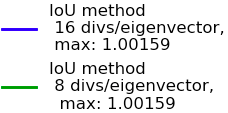
\includegraphics[scale = 0.41]{illImages/leg1.png}~
  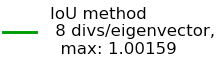
\includegraphics[scale = 0.41]{illImages/leg2.png}~
  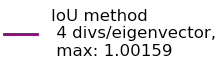
\includegraphics[scale = 0.41]{illImages/leg3.png}
  }
  \caption{Flowpipe bounds at different time points for
    Example~\ref{eg:ill}}
  \label{fig:ill}
\end{figure}
%
